\section{Preliminary Experiments}
\label{sec:experiment}
In this section, we did the experiments by comparing applying a model
checker to original C language programs with to abstracted
behavior. Figure~\ref{fig:statistic} shows the results of the
experiments. All of the experiments are done on a machine with an
Inter(R) Core i5-4590 3.30Hz CPU, 6MB cache and 8GB memory, running
Debian (kernel version) and CPAchecker (version 1.3.2).

In Figure~\ref{fig:statistic}, the meaning of each column is described
as follows. There are mainly two columns, \texttt{original programs}
and \texttt{abstracted behavior}, which means applying the model
checker to a original C language program and to abstracted behavior
respectively. These two columns consist of several columns:
$\sharp$\texttt{loc} means the number of program locations;
$\sharp$\texttt{fun} means the number of functions in a program;
\texttt{cpu time (total)} means the total execution time of CPU in
seconds; \texttt{memory(MB)} means the number of virtual memory cells
consumed by model checker in \texttt{MByte}; \texttt{fixed num} means
the number of available memory cells which we fix; the \texttt{true}
or \texttt{false} behind \texttt{fixed num} means it is \texttt{true}
if the number of the memory cells which a program consumes does not
exceed the \texttt{fixed num}, otherwise it is \texttt{false}.

The programs used for the experiments are described as follows:[TODO]
\begin{itemize}
\item \texttt{linklist.c} and \texttt{linklist2.c} create a list,
\item \texttt{linkstack.c} creates a stack.
\item \texttt{linkqueue.c} creates a queue.
\item \texttt{binarysorttree.c} sorts a binarytree
\item \texttt{database.c} creates a database.
\item \texttt{ihex2fw.c} is a file from Linux kernel
  \texttt{/firmware/ihex2fw.c}, which converts ihex files into binary
  representation for use by Linux kernel.
\item \texttt{gen\_init\_cpio.c} is a file from Linux kernel
  \texttt{/usr/gen\_init\_cpio.c}, which produces a binary file which
  performs on a file containing newline separated entries that
  describe the files to be included in the initramfs archive.
\end{itemize}

The results present in the Figure~\ref{fig:statistic} show that the
resources required for model checking become smaller if applying model
checkers to the abstracted behavior, since the abstracted behavior
only consists of allocation and deallocation.

One thing we should notice in Figure~\ref{fig:statistic} is that
the
result of \texttt{true} or \texttt{fals}e in the\texttt{fixe num} column may
be different for the same program, for example, linklist.c has the
true under original column but the false under behavioral column,
because

\begin{figure}
 \centering
 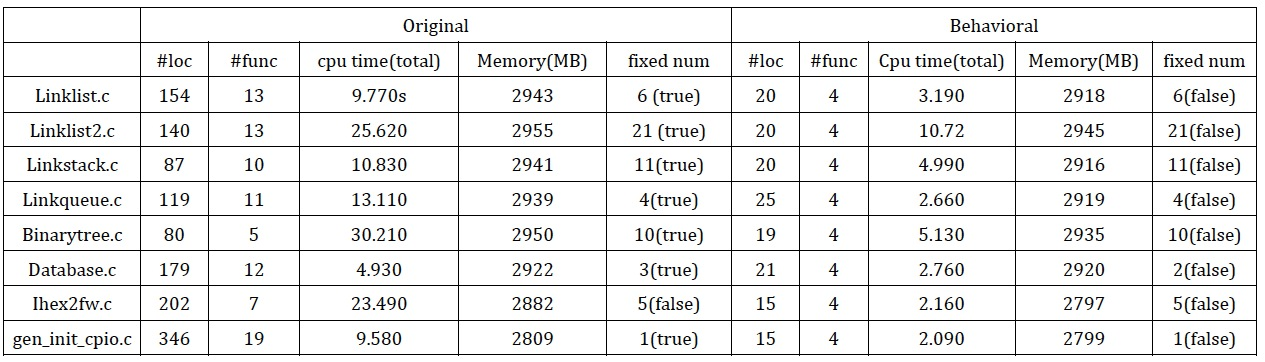
\includegraphics[width=14cm]{statistic.png}
\caption{Comparison}
\label{fig:statistic}
\end{figure}
